\documentclass[12pt]{unlsilabsop}
\title{Thermal and electrical resistance measuremets}
\date{May 6, 2019}
\author{Jose Andres Monroy}
\approved{Jose Andres Monroy}
\sopid{001}
\sopversion{v1}
\sopabstract{Describes the procedures to meassure the thermal resistance of the mock modules.}
\begin{document}

\maketitle

%------------------------------------------------------------------
\section{Scope}
This is regular procedure during the TFPX Phase II R\&D stage.

%------------------------------------------------------------------
\section{Purpose}
Determination of the thermal resistance is fundamental to characterize the cooling process; in particular to model the thermal runaway (more details needed here). This document describes the procedure followed to determine the Electrical resistance and thermal resistance of the module. The procedure can be extended in case of measuring the thermal resistance of a stack of materials like module+graphite+XXX.

%------------------------------------------------------------------
%>\section{Definitions}

%------------------------------------------------------------------
\section{Intro}
When the module is  
\begin{itemize}
    \item xxx
\end{itemize}

%------------------------------------------------------------------
\section{Equipment}

\begin{itemize}
    \item TDK-Lambda power supply (Z+).  
    \item Cables
    \item Digital Multmeters (DVM)
    \item Bread board
    \item Mock module (module)
    \item FLIR E50 IR camera (including tripod) (IRcam)
    \item Laptop
\end{itemize}

%------------------------------------------------------------------
\section{Procedure}
\begin{enumerate}
    \item Mount the circuit according to the schematic in Figure \ref{Rm_circuit} left.
    \item Mount the module on the brace of the support as shown in Figure \ref{Rm_circuit} right.
    \item Mount the IRcam, turn it on and locate it such that the module appears in the center of the field of view of the camera.
        \begin{figure}[h!]
          \begin{center}
          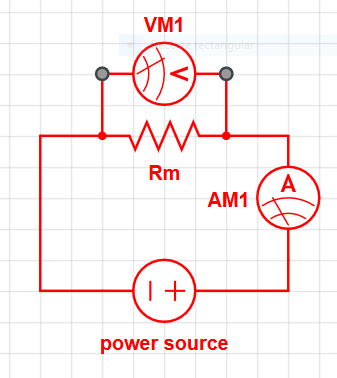
\includegraphics[width=0.3\textwidth]{img/Rm_circuit.png}\\
          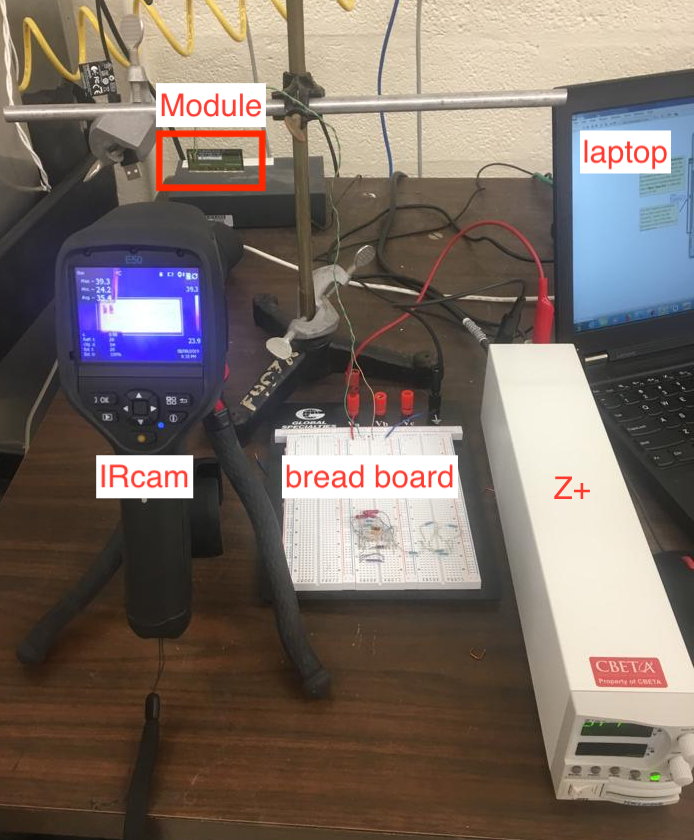
\includegraphics[width=0.8\textwidth]{img/setup.png}
          \caption{Electrical and Thermal resistance measurement circuit and setup.}
          \label{Rm_circuit}
          \end{center}
        \end{figure}
    \item Check that the IRcam is set to measure the minimum, average and maximum tmperatures; The IRcam screen should looks like the image in figure \ref{ircam_setup} left.  
      \begin{center}
        \begin{figure}[h!]
          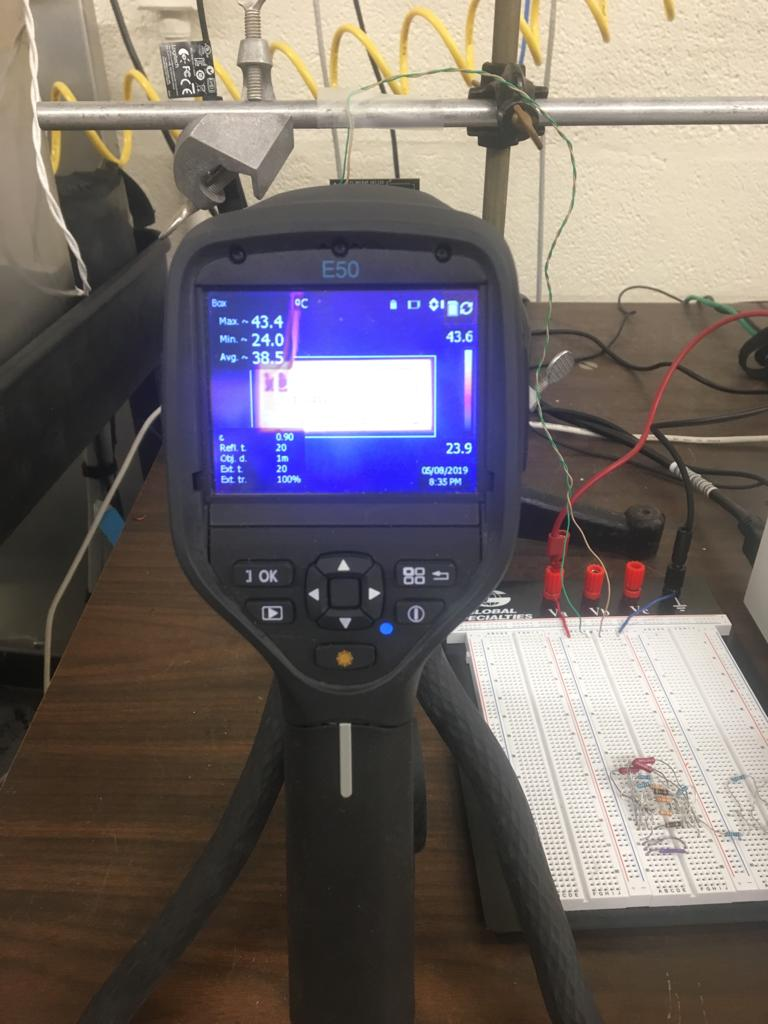
\includegraphics[width=0.5\textwidth]{img/ircam_setup}
          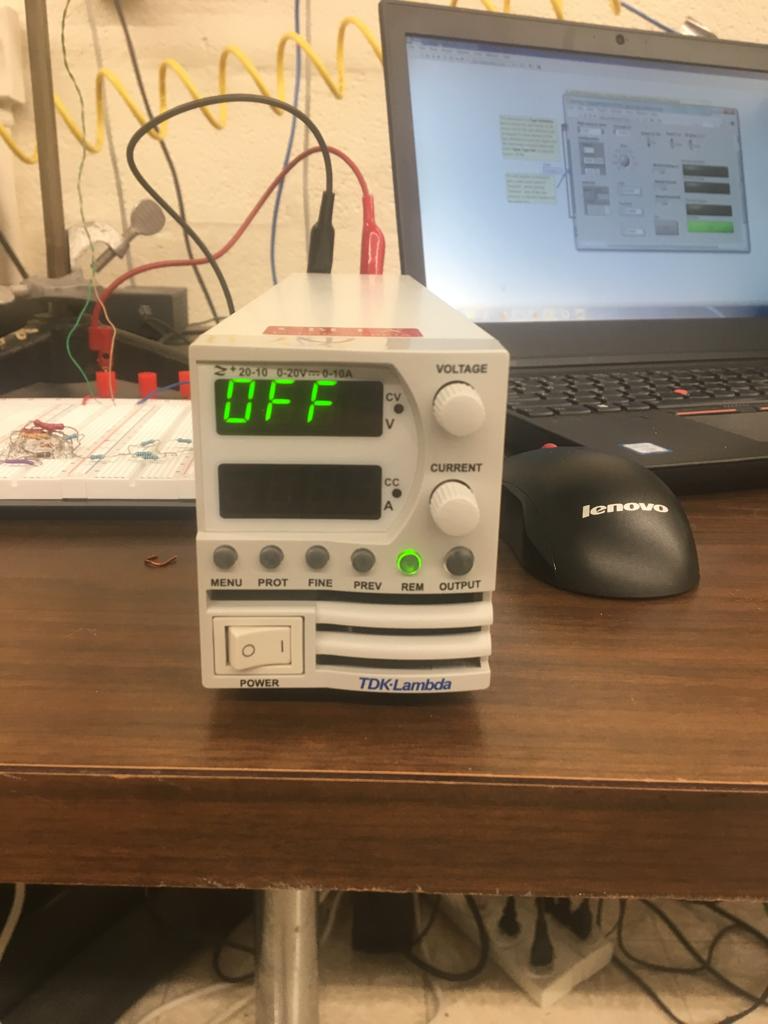
\includegraphics[width=0.5\textwidth]{img/z+.png}
          \caption{.}
          \label{ircam_setup}
        \end{figure}
      \end{center}
    \item Prepare an excel-spreadsheet or file to collect the values of: voltage and current as measured by the DVM and Z+ led indicators, minimum, average and maximun temperatures, timestamp. 
    \item Turn on the Z+; the indicators will blink for about two seconds, then, the upper led indicator will show OFF and the REM indicator will be on permanently (see figure \ref{ircam_setup} right). 
    \item The Z+ output is controlled by a Labview program called "$thermal_runaway_power.vi$". The basic funcionality allows the user to change the Voltage output (Vi) (the current change according to the Ohm's law) and so the power while keeping fixed the temperature; Open the program and check the initial conditions as shown in figure \ref{trp_lv}
      \begin{center}
        \begin{figure}[h]
          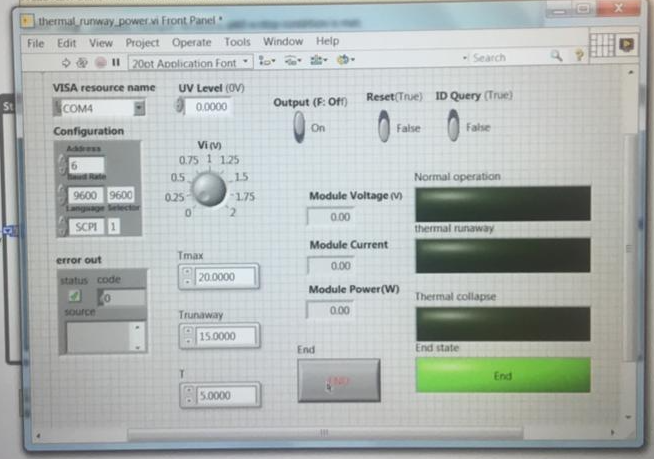
\includegraphics[width=\textwidth]{img/trp_lv1.png}
          \caption{.}
          \label{trp_lv}
        \end{figure}
      \end{center}
    \item Run the program; now the led indicators should show 0.00 and CV led to the right should be on (see Figure \ref{data.png}). Collect measurements: voltages, currents, temperatures, timestamp.
    \item Adjust the voltage to 0.20 using the voltage control (Vi) in the Labview front panel. Collect the Voltage and curent measurements (these would be stable) while the temperatures would start to increase, so wait for 10-15 minutes for stabilization and start taking temperature measurements every minute until full stabilization of the temperature (it may take about 40 minutes in total). Check that voltages and currents are stable, if not, collect those values in the table too.  
      \begin{center}
        \begin{figure}[h]
          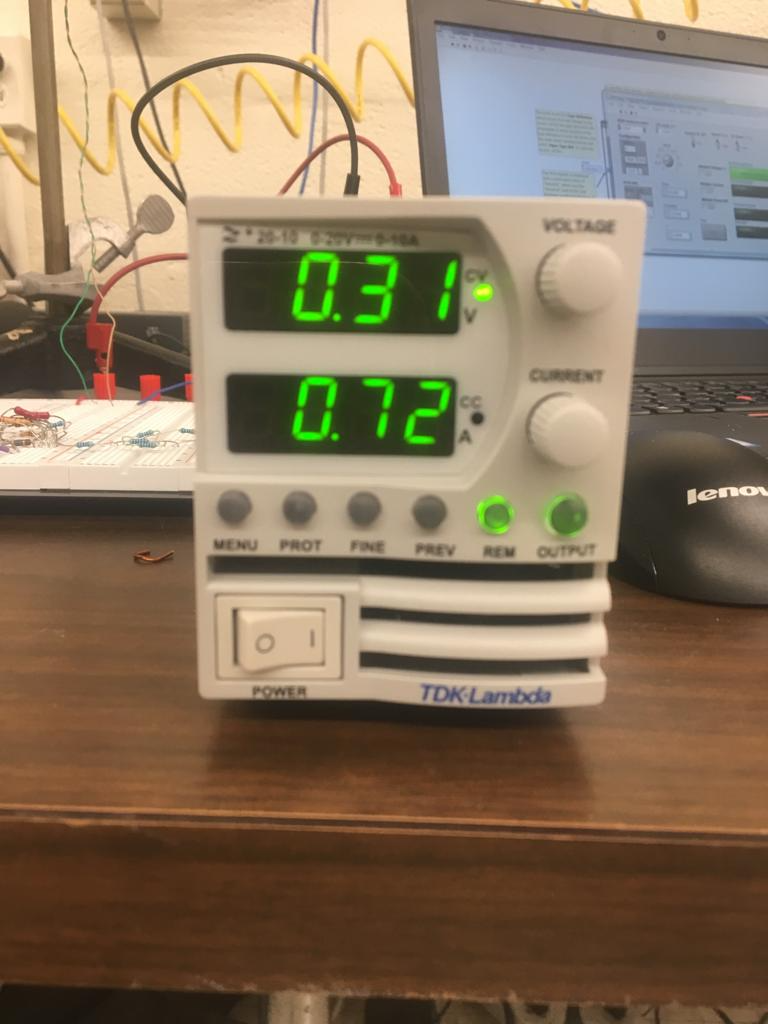
\includegraphics[width=0.5\textwidth]{img/data1.png}
          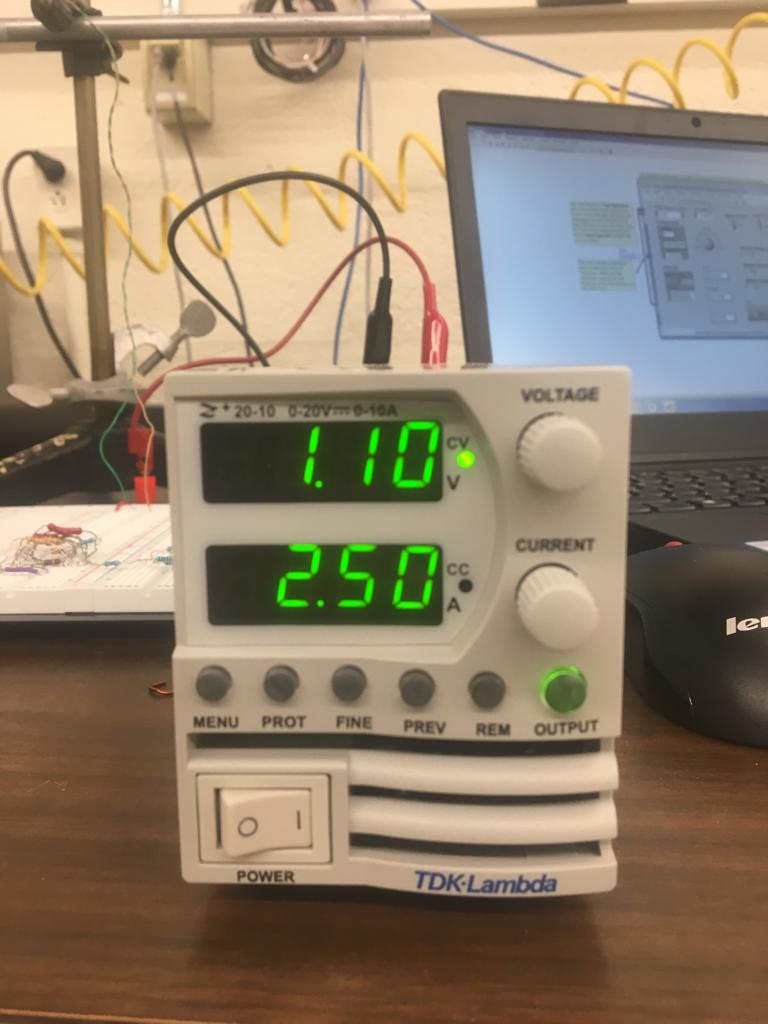
\includegraphics[width=0.5\textwidth]{img/data2.png}
          \caption{.}
          \label{data}
        \end{figure}
      \end{center}
    \item repeat the previous step until output voltage Vi= 2V.
    \item hit "End" button in the front panel to finish the Labview execution.
    \item Save data files as a "comma separated values" CSV file.
    \item turn off the IRcam and Z+.
\end{enumerate}

Analize data to extract the electrical and thermal resistance of the modules.

%------------------------------------------------------------------
\section{Documentation}
Everything needs to be documented in a report.

\end{document}

